\documentclass[11pt,a4paper]{article}

\setlength{\topmargin}{0cm}
\setlength{\headheight}{0.4cm}
\setlength{\headsep}{0.8cm}
\setlength{\footskip}{1cm}
\setlength{\textwidth}{17cm}
\setlength{\textheight}{25cm}
\setlength{\voffset}{-1.5cm}
\setlength{\hoffset}{-0.5cm}
\setlength{\oddsidemargin}{0cm}
\setlength{\evensidemargin}{0cm}
\setlength{\parskip}{6pt}



\usepackage[latin1]{inputenc}
\usepackage[cyr]{aeguill}
\usepackage[francais]{babel}
\usepackage[T1]{fontenc}
\usepackage{amsmath}
\usepackage{amssymb} %symboles math
\usepackage{amsfonts} %symboles math 
\usepackage{enumitem}
\usepackage{tikz} 
\usepackage{float}
\usepackage{braket}
\usepackage{fancyvrb}
\usepackage{minted}
\usepackage{graphicx} 
\usepackage{fancyhdr} 
\usepackage{epstopdf} 
\usepackage[squaren,Gray]{SIunits}
\usepackage{tabularx} % gestion avancée des tableaux
\usepackage{url}
\usepackage{hyperref}
\usepackage{bbold}
\usepackage[format=hang]{caption}
\usepackage{subcaption}
\usepackage{stmaryrd} 
\usepackage{placeins} 


\usepackage{caption}

% faire du code python
\usepackage{listings}
\usepackage{color}
\definecolor{mygreen}{rgb}{0,0.6,0}
\definecolor{mygray}{rgb}{0.5,0.5,0.5}
\definecolor{mymauve}{rgb}{0.58,0,0.82}
\lstset{ %
  backgroundcolor=\color{white},   % choose the background color; you must add \usepackage{color} or \usepackage{xcolor}; should come as last argument
  basicstyle=\footnotesize,        % the size of the fonts that are used for the code
  breakatwhitespace=false,         % sets if automatic breaks should only happen at whitespace
  breaklines=true,                 % sets automatic line breaking
  captionpos=b,                    % sets the caption-position to bottom
  commentstyle=\color{mygreen},    % comment style
  deletekeywords={...},            % if you want to delete keywords from the given language
  escapeinside={\%*}{*)},          % if you want to add LaTeX within your code
  extendedchars=true,              % lets you use non-ASCII characters; for 8-bits encodings only, does not work with UTF-8
  frame=single,	                   % adds a frame around the code
  keepspaces=true,                 % keeps spaces in text, useful for keeping indentation of code (possibly needs columns=flexible)
  keywordstyle=\color{blue},       % keyword style
  language=Octave,                 % the language of the code
  morekeywords={*,...},            % if you want to add more keywords to the set
  numbers=left,                    % where to put the line-numbers; possible values are (none, left, right)
  numbersep=5pt,                   % how far the line-numbers are from the code
  numberstyle=\tiny\color{mygray}, % the style that is used for the line-numbers
  rulecolor=\color{black},         % if not set, the frame-color may be changed on line-breaks within not-black text (e.g. comments (green here))
  showspaces=false,                % show spaces everywhere adding particular underscores; it overrides 'showstringspaces'
  showstringspaces=false,          % underline spaces within strings only
  showtabs=false,                  % show tabs within strings adding particular underscores
  stepnumber=2,                    % the step between two line-numbers. If it's 1, each line will be numbered
  stringstyle=\color{mymauve},     % string literal style
  tabsize=2,	                   % sets default tabsize to 2 spaces
  title=\lstname                   % show the filename of files included with \lstinputlisting; also try caption instead of title
}



\pagestyle{fancy}
\fancyhead[L]{\scriptsize \textsc{Une méthode de calibration non paramétrique pour les calorimètres de CMS}}
\fancyhead[R]{\scriptsize \textsc{Samuel Niang}} 
\fancyfoot[C]{ \thepage}

% commande de déplacement d'un objet
\newcommand{\drawat}[3]{\makebox[0pt][l]{\raisebox{#2}{\hspace*{#1}#3}}}

\usepackage[printwatermark]{xwatermark}
\newwatermark[allpages,color=red!50,angle=45,scale=3,xpos=0,ypos=0]{DRAFT}

  
\begin{document}

% Pour faciliter la mise en forme de la page du titre, on supprime l'indentation automatique en début de paragraphe
\setlength{\parindent}{0pt}

\thispagestyle{empty}

\includegraphics[height=2cm]{images/logoens.eps} \hfill \includegraphics[height=2cm]{images/logoucbl.eps} \hfill \includegraphics[height=2cm]{images/logounivlyon.png}

\vspace{1cm}

\begin{tabularx}{\textwidth}{@{} l X l @{} }
{\sc Master Science de la matière} & & Rapport de stage\\
{\it \'{E}cole Normale Supérieure de Lyon} & & Samuel Niang\\
{\it Université Claude Bernard Lyon I} & & M2 Physique - Concepts et applications

\end{tabularx}


\begin{center}

\vspace{1cm}

\rule[11pt]{5cm}{0.5pt}

\textbf{\huge Une méthode de calibration non paramétrique pour les calorimètres de CMS.}

\rule{5cm}{0.5pt}

\vspace{2cm}

\parbox{15cm}{\small
\textbf{Résumé} : \\
\rm Dans le détecteur CMS, l'énergie des hadrons neutres est déterminée à partir de l'énergie mesurée dans les calorimètres électromagnétiques ($E_{\rm ecal}$) et hadroniques ($E_{\rm hcal}$). Une calibration est cependant nécessaire pour estimer l'énergie vraie du hadron neutre à partir de $E_{\rm ecal}$ et $E_{\rm hcal}$. Dans un premier temps, j'ai utilisé comme calibration une fonction linéaire de $E_{\rm ecal}$ et $E_{\rm hcal}$. Ensuite, afin de décrire la non linéarité de la mesure de l'énergie, j'ai inventé une nouvelle méthode de calibration non paramétrique.
}

\vspace{1cm}
\begin{center}
\includegraphics[height=2cm]{images/Logo_IPNL.jpg} 
\hspace{1cm}
\includegraphics[height=2cm]{images/Logo_CMS.png} 
\hspace{1cm}
\includegraphics[height=2cm]{images/cern_logo.png} 
\end{center}
\vspace{1cm}

\parbox{15cm}{
\textbf{Mots clefs} : \it Calibration, Modélisation, Physique des particules
} 

\vspace{0.5cm}

\parbox{15cm}{
Stage encadré par :

{\bf Colin Bernet}
\href{mailto:colin.bernet@cern.ch}{\tt colin.bernet@cern.ch} 

%Nom du Laboratoire d'accueil

{\it Bâtiment Paul Dirac\\
4, Rue Enrico Fermi\\
69622 Villeurbanne Cedex\\
Tél. : +33 (0) 4 72 44 84 57}

} %fin de la commande \parbox encadrant / laboratoire d'accueil

\vspace{0.5cm}

\end{center}
\vfill
\hfill \today

\newpage
\thispagestyle{empty}
\tableofcontents
\setcounter{page}{1}

\setlength{\parindent}{16pt}





\newpage
\section{Introduction}
Après avoir permis la découverte expérimentale du boson de Higgs en 2012, les expériences généralistes ATLAS \cite{HiggsATLAS} et CMS \cite{HiggsCMS} installées sur le LHC du CERN, sont toujours en place dans l'optique de découvrir de la nouvelle physique au-delà du modèle standard.

Les détecteurs ATLAS et CMS sont basés sur les mêmes principes : cylindriques, ils sont constitués d'un ensemble de sous-détecteurs disposés en couches concentriques autour du point d'interaction. Les informations provenant de ces sous-détecteurs sont combinées pour déterminer le type, l'énergie et la direction des particules de l'état final de la collision, pour pouvoir mesurer les propriétés de celle-ci, et par exemple déterminer si une particule instable encore inconnue a été produite. 

Nous allons nous intéresser plus spécifiquement au détecteur CMS \cite{CMS}. Celui-ci dispose  :
\begin{itemize}
\item d'un champ magnétique, pour courber la trajectoire des particules chargées;
\item d'un trajectographe, pour reconstruire la trajectoire des particules chargées, et ainsi obtenir la charge et l'impulsion;
\item d'un calorimètre électromagnétique (ECAL) \cite{ECAL}, constitué d'un cristal de tungstate de plomb, permettant de collecter les dépôts d'énergie des particules, principalement électrons et photons, mais aussi hadrons chargés et neutres;
\item d'un calorimètre hadronique (HCAL) \cite{HCAL}, composé de plusieurs couches d'absorbeur en laiton et de carreaux scintillateurs en plastique, avec une segmentation grossière. La resolution du HCAL pour la mesure de l'energie $E$ d'un hadron est de l'ordre de $100\%\sqrt{(E / \SIUnits{}{\giga\electronvolt})}$;
\item de chambres à muons, qui permettent l'dentification de ces particules, les seules à pouvoir y parvenir.
\end{itemize}

\begin{figure}[!h]
\begin{center}
\includegraphics[width=0.7\textwidth]{images/detecteur.pdf}
\caption{Une esquisse des interactions spécifiques des particules dans une tranche transversale du détecteur CMS.}
\label{schemaCMS}
\label{detecteur}
\end{center}
\end{figure}

Détaillons alors le comportement des particules  :
\begin{itemize}
    \item photons (exemple 1 dans la Fig. \ref{schemaCMS}) :
    	\begin{itemize}
		\item déposent leur énergie dans ECAL;
	\end{itemize}
    \item $e^+,e^-$ (exemple 2 dans la Fig. \ref{schemaCMS}) :
        \begin{itemize}
        		\item produisent une trace dans le trajectographe;
		\item déposent leur énergie dans ECAL;
        \end{itemize}
    \item hadrons chargés (exemple 3 dans la Fig. \ref{schemaCMS}) :
        \begin{itemize}
        		\item produisent une trace dans le trajectographe;
    		\item déposent en minorité des cas leur énergie dans ECAL;
    		\item déposent leur énergie dans HCAL;
		\item finnissent leur course dans HCAL;
        \end{itemize}
    \item hadrons neutres (exemple 4 dans la Fig. \ref{schemaCMS}) :
        \begin{itemize}
        		\item déposent leur énergie dans le HCAL;
		\item déposent dans la minorité des cas leur énergie dans ECAL;
		\item finnissent leur course dans HCAL;
        \end{itemize}
    \item $\mu^+,\mu^-$ (exemple 5 dans la Fig. \ref{schemaCMS}) :
        \begin{itemize}
        		\item produisent une trace dans le trajectographe;
		\item traversent ECAL, HCAL;
		\item sont visibles dans la chambre à muons.
        \end{itemize}
\end{itemize}
\`A noter que dans notre étude, seuls les hadrons neutres nous intéressent. \\

La connaissance des dépôts d'énergie et du comportement des particules dans les différentes parties du détecteur nous permettent de reconnaître et distinguer les particules : cette opération s'appelle le \textit{Particle Flow (PF)}. Cependant, il est aussi nécessaire d'estimer l'énergie des particules ($E_{\rm true})$ à l'aide d'une calibration des calorimètres. En effet, ces derniers ne présentent pas une réponse linéaire et la somme des énergies dans les calorimètres ne correspond pas à l'énergie de la particule. Cette énergie de calibration sera notée $E_{\rm calib}$.

En première approximation, nous déterminerons l'énergie calibrée par une fonction linéaire de l'énergie lue dans le ECAL (énergie notée par la suite $E_{\rm ecal}$) et de celle lue dans le HCAL (notée par la suite $H_{\rm ecal}$). Cette méthode sera présentée dans la section \ref{LR}.

Ce rapport présente ensuite de nouvelles techniques de calibration qui permettent de prendre en compte la non-linearité des calorimètres. Ces techniques seront présentées dans les sections \ref{CL} et \ref{KNN}.\\
Enfin, nous comparerons ces méthodes dans la section \ref{comparaison}. 

\section{Production de l'échantillon}

\begin{figure}[!h]
\begin{center}
\includegraphics[height=5cm]{images/pictures/testLinearRegression/LinearRegression_plot3D_training.png}
\caption{Le nuage de points $(E_{\rm ecal},E_{\rm hcal}, E_{\rm true})$}
\end{center}
\end{figure}

- paragraphe de Colin sur la simulation\\

Les données simulées sont stockées dans un fichier \textit{.root}. Par souci de compatibilité, j'ai voulu écarter \textit{Root}, qui est à  la fois un programme et une librairie C++ pour tout faire en Python.  J'ai donc écrit un programme \cite{RootToPhython} pour extraire les données du fichier initial pour les déplacer dans un nouveau fichier binaire importable facilement par Python et qui contient, pour chaque hadron simulé : son énergie réelle ($E_{\rm true}$), son impulsion, l'énergie déposée dans ECAL ($E_{\rm ecal}$), l'énergie déposée dans HCAL ($E_{\rm hcal}$), sa pseudo-rapidité.

On séparera et traitera différemment les événements qui ont $E_{\rm ecal} = 0$.  Ces événements sont liés à des particules qui ont interagi avec le détecteur hardronique mais pas avec le détecteur électromagnétique (cf Fig.\ref{detecteur}). Cette séparation se justifie, car modéliser les dépôts d'énergie dans les deux calorimètres pour en conclure ce qui se passe dans le cas particulier où il n'y a de dépôt que dans l'un d'eux amène un biais. Ainsi, à chaque construction de calibration, on créera en fait deux modèles.

De plus, la simulation crée un palier car les particules sont limitées à $E_{\rm true} = \SIUnits{200}{\giga\electronvolt}$? Si l'on regarde par exemple sur la Fig. \ref{limite} ce qui se passe dans le plan $E_{\rm ecal} = 0$, on voit bien ce palier qui apparaît vers $\SIUnits{150}{\giga\electronvolt}$, il est donc ici impossible de déduire une énergie de calibration à partir des points au-delà de cette limite . Avec ce jeu de données, nous allons fixer une limite $E_{\rm ecal} + E_{\rm hcal}$  = (lim = \SIUnits{150}{\giga\electronvolt})$.

\begin{figure}[!h]
    \begin{center}
        \includegraphics[width=\textwidth]{images/pictures/explain/limit_arrow.png}
        \caption{On place une limite à $E_{\rm ecal}+E_{\rm hcal} = 150$. Les points verts sont les points rejetés.}
        \label{limite}
    \end{center}
\end{figure}

\section{Calibration par régression linéaire}
\label{LR}

Comme première calibration, j'ai utilisé une méthode simple, la régression linéaire. Il s'agit de supposer qu'il existe une relation 
\begin{equation}
    E_{\rm true} = a_1 E_{\rm ecal} + a_2 E_{\rm hcal} + b
\end{equation}
et de trouver les coefficient $a_1, a_2,  b$ optimaux pour que le modèle coïncide au mieux aux données d'entrainement. Au niveau de la programmation, j'ai utilisé la librairie de \textit{Sciki Learn}  \cite{scikitLR} qui se base sur une méthode des moindres carrés. Dans notre cas, cela revient à trouver les coefficients qui, pour un ensemble de données d'entraînement  $(E_{\rm ecal}^n,E_{\rm hcal}^n, E_{\rm true}^n)$ minimiseront :
\begin{equation}
	\epsilon = \sum_n |E_{\rm true} - a_1 E_{\rm ecal} - a_2 E_{\rm hcal} - b|^2
\end{equation}

J'ai constaté qu'à faible  $E_{\rm ecal},  E_{\rm hcal}$ il y a quelques points à très haut $E_{\rm true}$ qui correspondent à des défauts de la détection des énergies dans les calorimètres, je les ai donc enlevés des données d'entraînement pour la regression linéaire (cf Fig. \ref{selectedpoints}).

\begin{figure}[!h]
    \begin{center}
        \includegraphics[width=\textwidth]{images/pictures/testLinearRegression/LinearRegression_selectedpoints.png}
        \caption{En bleu, les points sélectionnés pour faire la régression linéaire.}
        \label{selectedpoints}
    \end{center}
\end{figure}

\begin{minipage}{0.65\linewidth}
    Nous pouvons à présent effectuer la regression linéaire sur un premier jeu de donné d'entrainement \cite{GitHubLR}  en ne prenant en compte dans la régression que les points tels que $ $\rm{lim_{\rm min}} < E_{\rm ecal} + E_{\rm hcal} < \rm{lim_{\rm max}}$, avec $\rm{lim_{\rm min}} = 10,\rm{lim_{\rm min}} = 150 $. Nous obtenons alors :
    \[
    \begin{cases}
    E_{\rm calib} =  0.95359395 E_{\rm hcal}  + 5.9057809 & E_{\rm ecal} = 0 \\
    E_{\rm calib} = 0.9876819  E_{\rm hcal}   + 1.3081561  E_{\rm ecal} + 8.5016036 & E_{\rm ecal} \neq 0
    \end{cases}
	\]
\end{minipage}
\begin{minipage}{0.35\linewidth}
	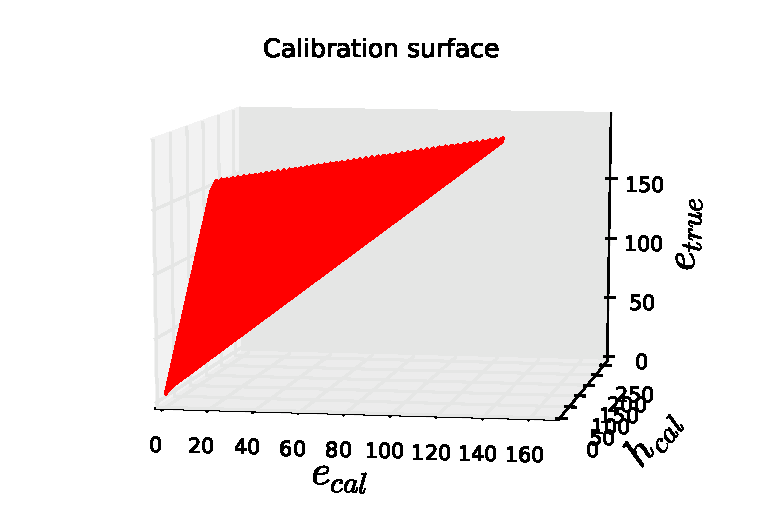
\includegraphics[width = \textwidth]{images/pictures/testLinearRegression/LinearRegression_plot3D_surf.eps}
	\captionof{figure}{Nuage de points modélisé par un plan}
\end{minipage}

\begin{figure}[!h]
\begin{center}
\includegraphics[height =5cm]{images/pictures/testLinearRegression/LinearRegression_calibration.png}
\caption{Courbe de calibration pour $E_{\rm ecal} = 0$.}
\end{center}
\end{figure}

Nous constatons en particulier que dans le cas  $E_{\rm ecal} = 0$, la courbe ne passe pas par le le coeur du nuage de point à faible  $E_{\rm hcal} = 0$. Maintenant que la régression est faite, nous allons calibrer un second jeu de données et afficher $E_{\rm calib}/$E_{\rm true}$ pour ce nouveau jeu de données. $E_{\rm calib}/$E_{\rm true}$ doit être le plus proche possible de 1.

Sur la Fig. \ref{LR_ecaliboveretrue_ecal_hcal}, à gauche, nous constatons comme prévu que la régression linéaire est mauvaise à faible $E_{\rm hcal}$ car en moyenne, $E_{\rm calib}/E_{\rm true}$ n'est pas proche de $1$. Plus intéressant, la figure de droite met en avant les non-linéarités du nuage de point.\\

\begin{figure}[!h]
\begin{center}
\includegraphics[height =4.5cm]{images/pictures/testLinearRegression/LinearRegression_ecalib_over_etrue_functionof_ecal_hcal.png}
\caption{$E_{\rm calib}/E_{\rm true}$ en fonction de $E_{\rm ecal}$ et $E_{\rm hcal}$.}
\label{LR_ecaliboveretrue_ecal_hcal}
\end{center}
\end{figure}


Sur la Fig. \ref{LR_ecaliboveretrue_etrue} nous constatons également que la calibration dévie : $E_{\rm calib}/E_{\rm true}$  est trop écarté de 1.
\begin{figure}[!h]
\begin{center}
\includegraphics[height =4.5cm]{images/pictures/testLinearRegression/LinearRegression_ecalib_over_etrue.png}
\caption{$E_{\rm calib}/E_{\rm true}$ en fonction de $E_{\rm true}$.}
\label{LR_ecaliboveretrue_etrue}
\end{center}
\end{figure}

Il faut donc proposer une méthode qui prend en compte la non-linéarité entre les 3 variables. 



\section{Méthode non paramétrique binnée}
\label{CL}
\noindent
\begin{minipage}{0.60\linewidth}
Ici, l'idée est de découper le plan $(E_{\rm ecal},E_{\rm hcal})$ en carrés et de calculer la moyenne des $E_{\rm true}$ dans chaque carré qui sera la valeur $E_{\rm calib}$. Ainsi pour prédire une énergie de $E_{\rm calib}^i$ pour un point $(E_{\rm ecal}^i,E_{\rm hcal}^i)$, nous allons regarder dans quel carré il se trouve et retourner la valeur d'énergie calibrée correspondante. Nous pouvons voir sur la Fig. \ref{legos} une illustration où la hauteur de chaque brique correspond à l'énergie calibrée d'un carré.
\end{minipage}
\begin{minipage}{0.4\linewidth}
	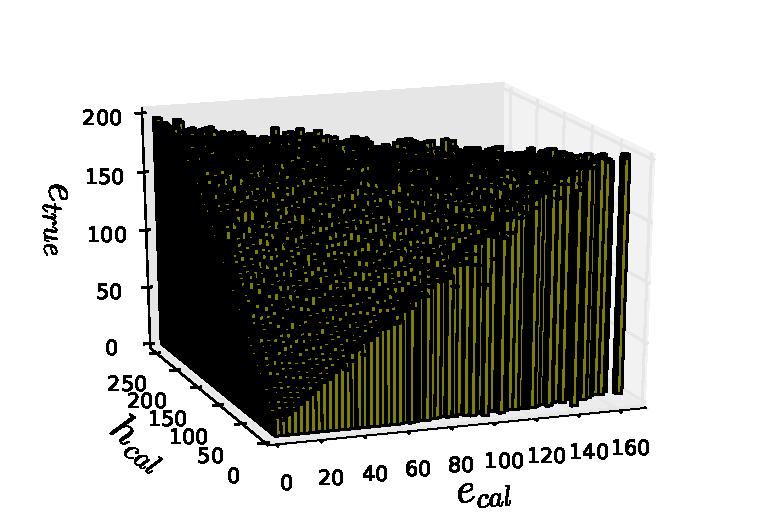
\includegraphics[width=\linewidth]{images/pictures/testCalibrationLego/CalibrationLego_plot3D_legos.eps}
	\captionof{figure}{Illustration de la calibration avec $100\times100$ carrés.}
	\label{legos}
\end{minipage}

L'avantage de cette calibration est de prendre en compte ce qui se passe localement dans la distribution contrairement à la régression linéaire, mais elle a pour désavantage d'être liée au pas des carrés. Un pas trop grand fait perdre en précision, un pas trop petit laisse des trous dans la position des briques (cf Fig. \ref{legos}), et fait exploser le temps de calcul. 

\noindent
\begin{minipage}{0.60\linewidth}
Construisons la calibration \cite{GitHubCL} à l'aide d'un premier jeu de données, avec $100\times100$ carrés. Premièrement, nous constatons que la surface est "cabossée", et si nous regardons ce qui se passe dans le plan $E{\rm ecal} = 0$ (Fig. \ref{calibCL}), nous voyons que cette méthode binnée donne des énergies calibrées $E_{\rm calib}$ égales pour des ensembles de points, par paliers. Deuxièmement, nous constatons une fois de plus que la courbe de calibration ne passe pas par le coeur de la distribution à bas $E_{\rm hcal}$ : $E_{\rm calib}$ y est sur-évaluée.
\end{minipage}
\hfill
\begin{minipage}{0.4\linewidth}
	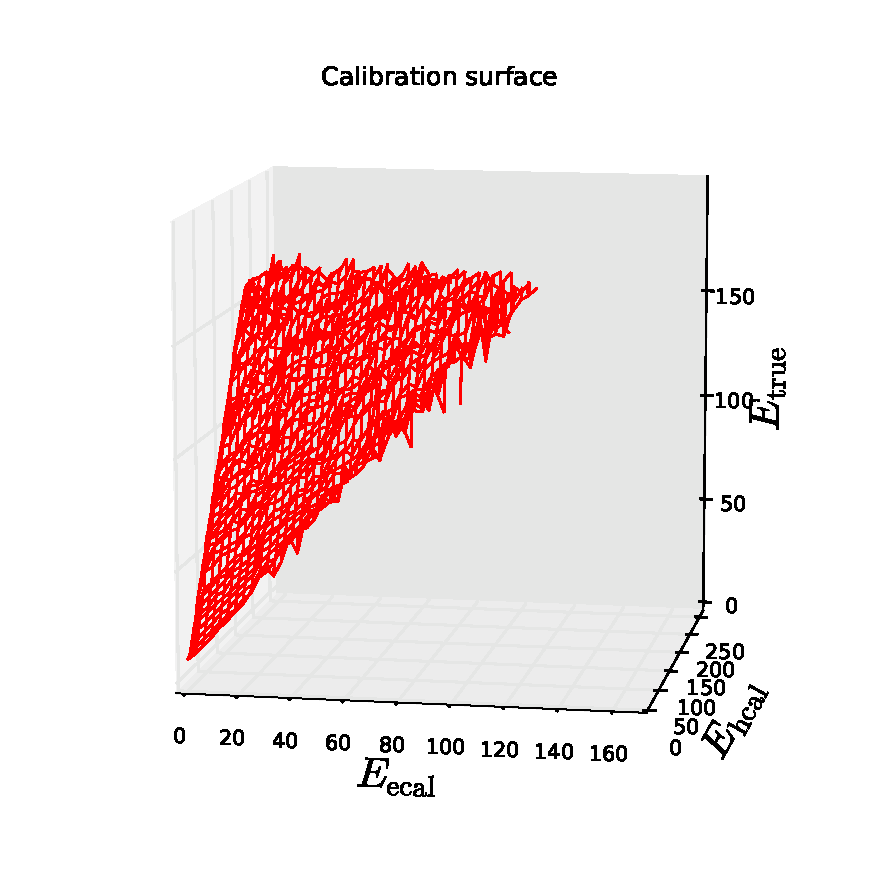
\includegraphics[width=\textwidth]{images/pictures/testCalibrationLego/CalibrationLego_plot3D_surf.eps}
	\captionof{figure}{Surface de calibration avec $100\times100$ carrés.}
	\label{legos}
\end{minipage}

\begin{figure}[!h]
\begin{center}
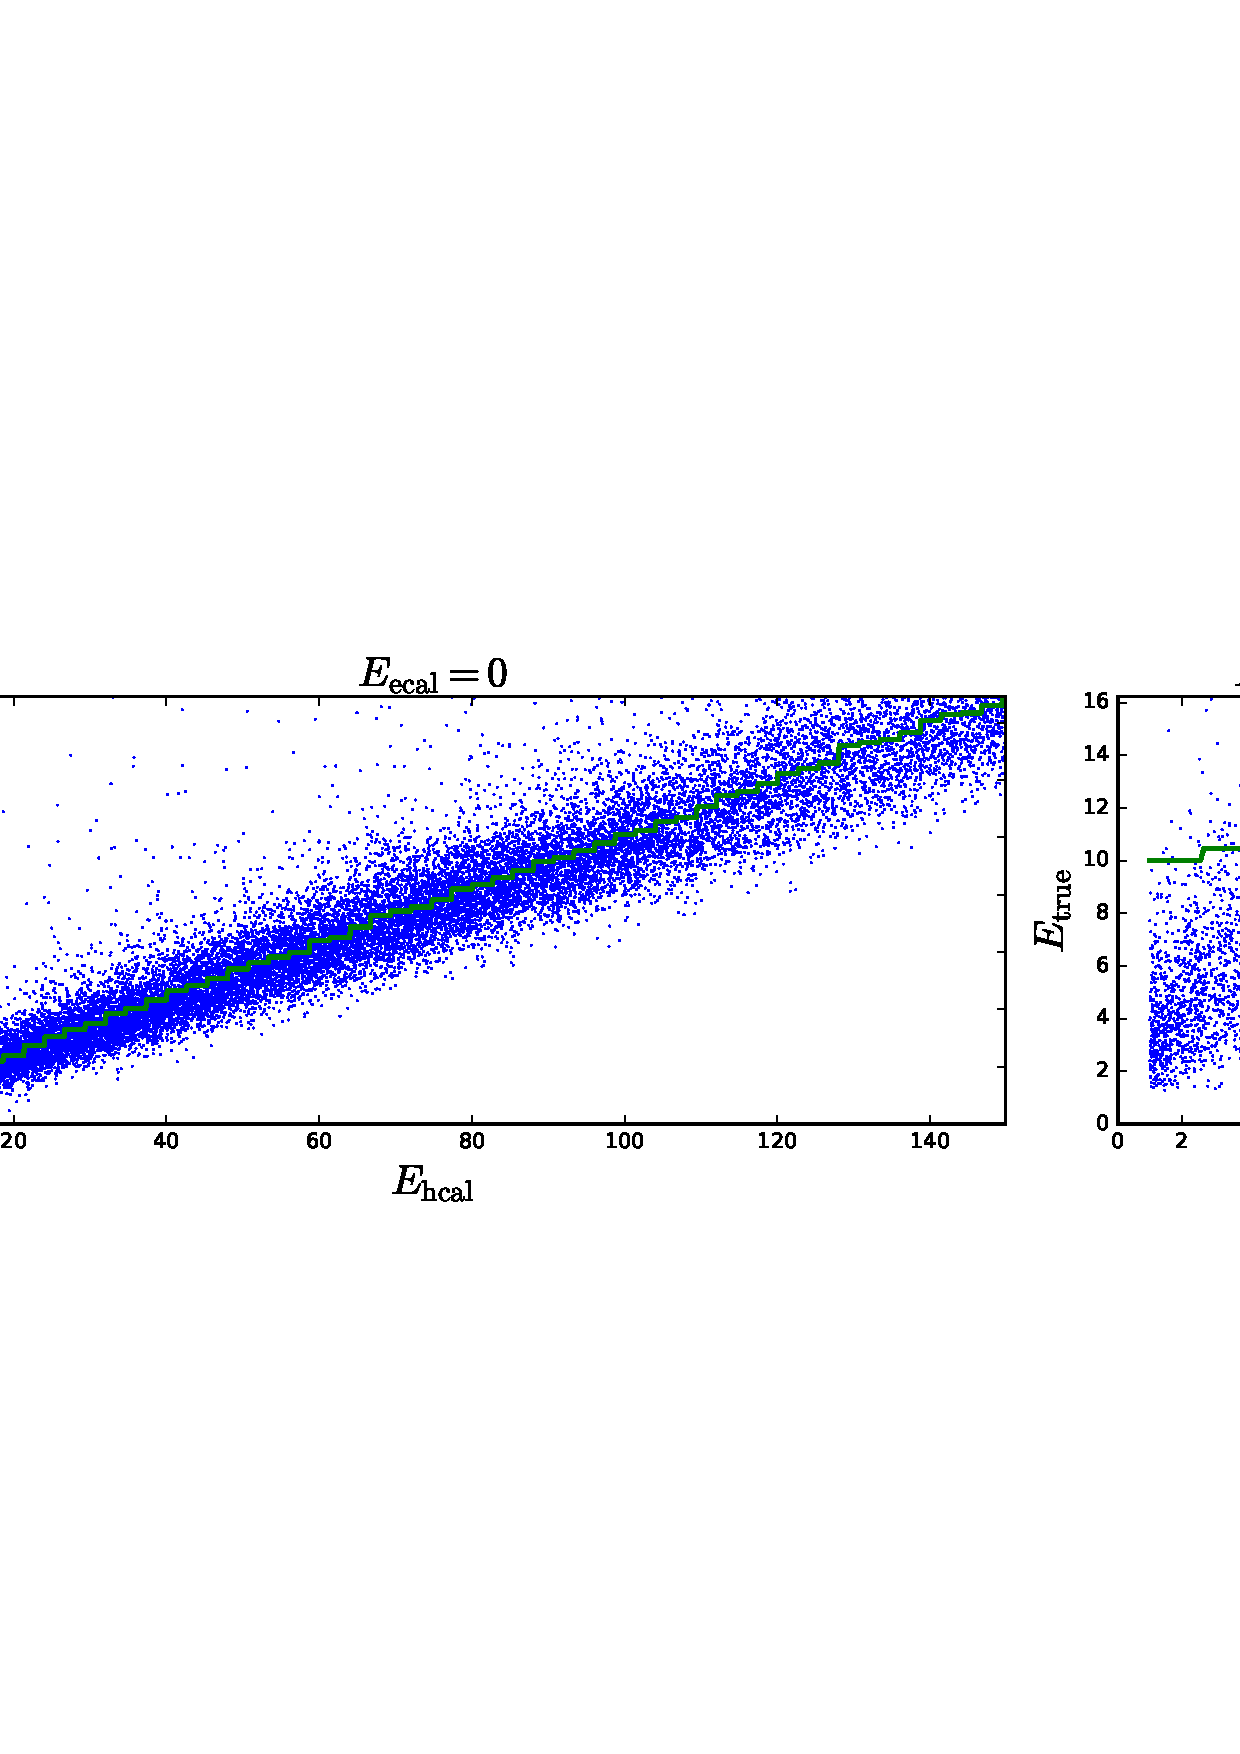
\includegraphics[width=\textwidth]{images/pictures/testCalibrationLego/CalibrationLego_calibration.png}
\caption{Courbe de calibration pour $E_{\rm ecal} = 0$.}
\label{calibCL}
\end{center}
\end{figure}

Effectuons la calibration d'un second jeu de données :
\begin{figure}[!h]
\begin{center}
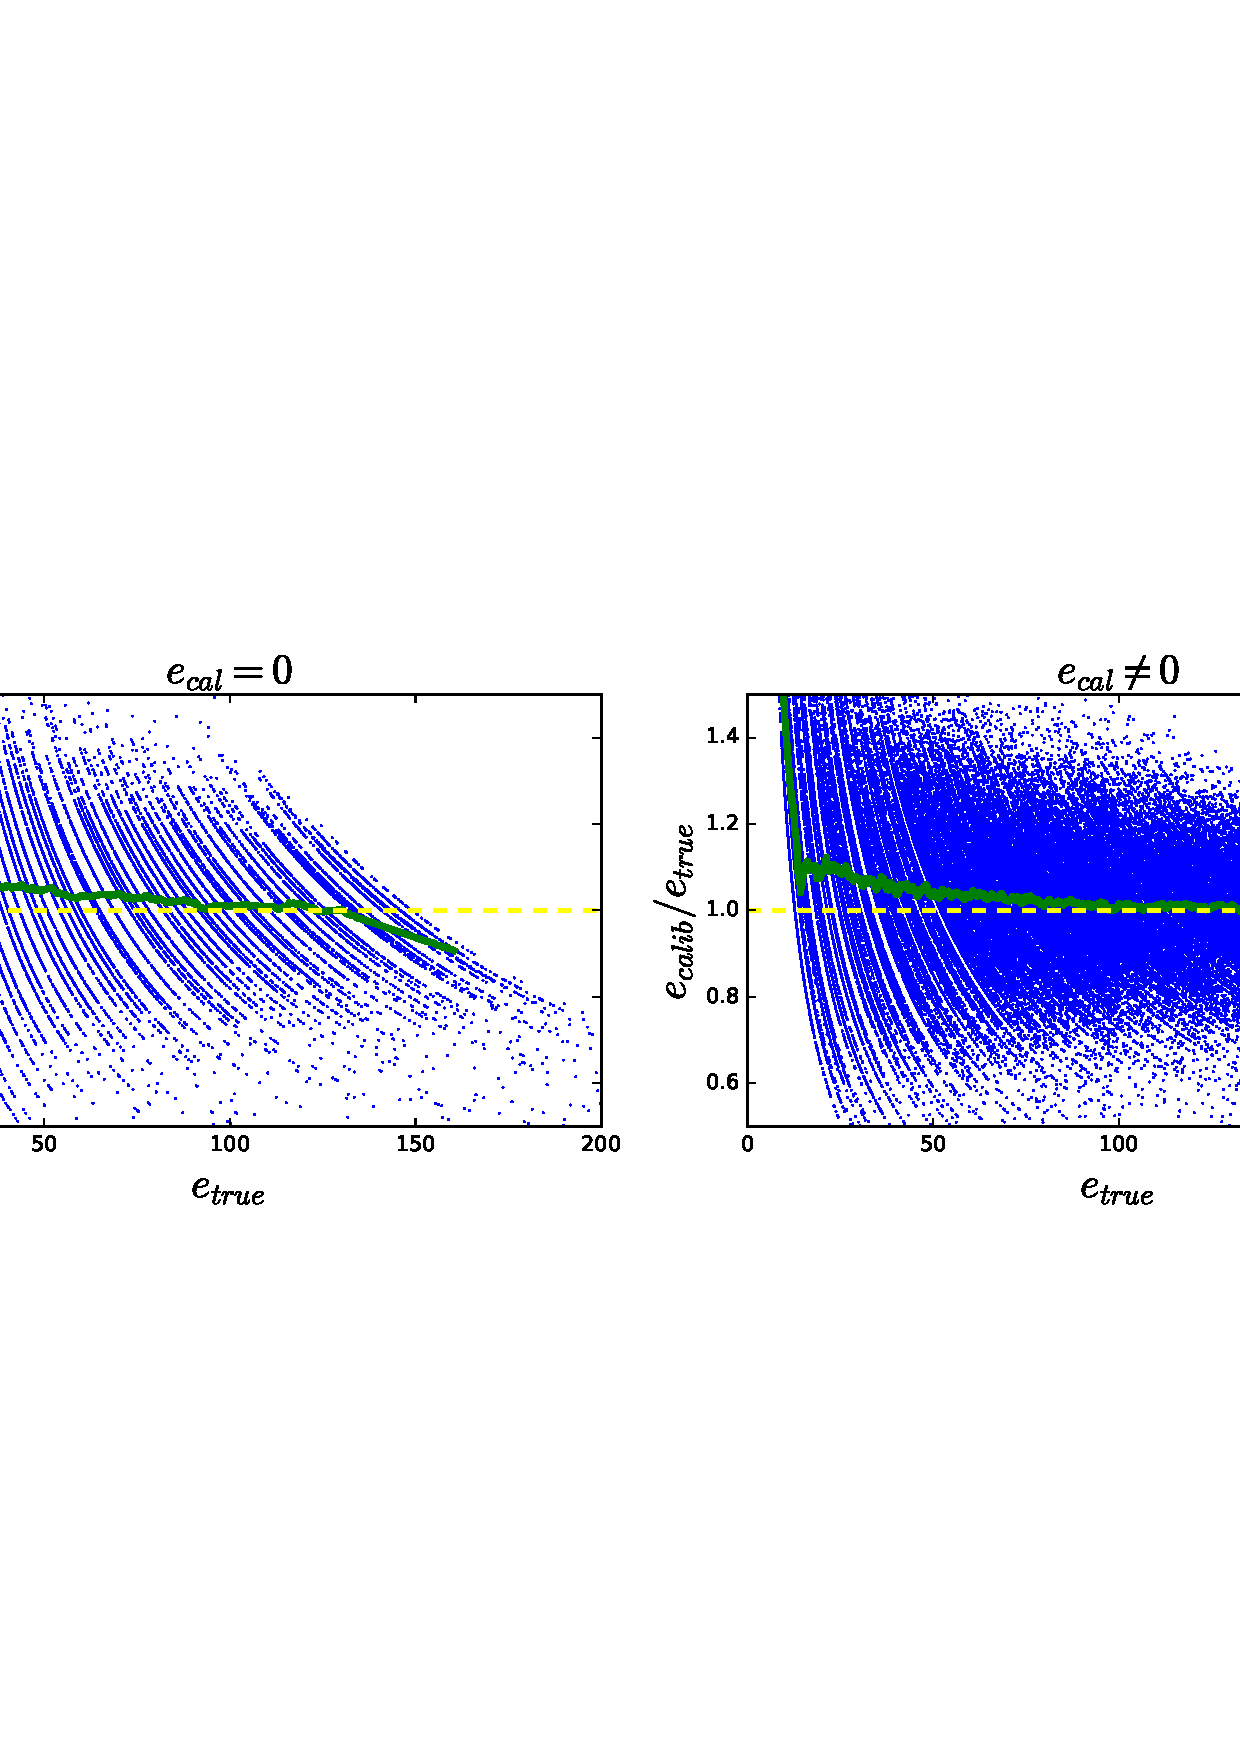
\includegraphics[width=\textwidth]{images/pictures/testCalibrationLego/CalibrationLego_ecalib_over_etrue.png}
\caption{$E_{\rm calib}/E_{\rm true}$ en fonction de $E_{\rm true}$. Nous voyons clairement l'apparition d'une structure, liée au caractère binné de la méthode.}
\label{ecaliboveretrueCL}
\end{center}
\end{figure}

Nous remarquons que la présence de paliers dans la courbe de calibration biaise la calibration en faisant apparaître une structure (des hyperboles) dans $E_{\rm calib}/E_{\rm true}$, comme nous pouvons le voir dans la Fig. \ref{ecaliboveretrueCL}. Cette structure est liée aux points possédant la même énergie de calibration, contrairement au cas de la régression linéaire (cf Fig.  \ref{LR_ecaliboveretrue_etrue}). 
Nous constatons également sur la Fig. \ref{ecaliboveretrueCL} que $E_{\rm calib}/E_{\rm true}$ est en moyenne constamment $> 1$, ce qui montre qu'il y a une tendance à la sur-évaluation de $E_{\rm calib}$.

\begin{figure}[!h]
\begin{center}
\includegraphics[width=\textwidth]{images/pictures/testCalibrationLego/CalibrationLego_ecalib_over_etrue_functionof_ecal_hcal.png}
\caption{$E_{\rm calib}/E_{\rm true}$ en fonction de $E_{\rm ecal}$ et $E_{\rm hcal}$.}
\label{ecaliboveretrueCL_etrue}
\end{center}
\end{figure}

La Fig. \ref{ecaliboveretrueCL_etrue} nous montre une fois de plus que $E_{\rm calib}/E_{\rm true}$  est globalement sur-évaluée, mais que cette fois-ci, nous avons pris en compte les non-linéarités. Il nous faut alors une méthode qui reprenne l'idée de moyenner des $E_{\rm true}$ en enlevant les contraintes et biais provenants des bins.

\section{Méthodes basées sur les plus proches voisins}
\label{KNN}
\subsection{Moyenne pondérée}
Nous utilisons encore des données simulées pour effectuer la calibration : chaque particule simulée $i$ est vue comme un point d'un espace tridimensionnel possédant des coordonnées $(E_{\rm ecal}^i, E_{\rm hcal}^i,E_{\rm true}^i)$.
Pour trouver l'énergie calibrée d'un point de coordonnées $(E_{\rm ecal}^0, E_{\rm hcal}^0)$ :
\begin{itemize}
	\item on recherche ses $k$ plus proches voisins dans le plan $(E_{\rm ecal}, E_{\rm hcal}) \rightarrow (E_{\rm ecal}^i, E_{\rm hcal}^i), i \in [|1,...,k|]$
	\item on effectue une moyenne pondérée des $E_{\rm true}^i$ de ces plus proches voisins $\rightarrow E_{\rm calib}^0$ : l'énergie calibrée.
\end{itemize}

La moyenne pondérée va donc s'exprimer ainsi :
\begin{equation}
	 E_{\rm calib}^0 = \frac{\sum_{i=1}^k g(E_{\rm ecal}^i, E_{\rm hcal}^i) \times E_{\rm true}^i}{\sum_{i=1}^k g(E_{\rm ecal}^i, E_{\rm hcal}^i)}
\end{equation}
Dans notre cas nous avons pris pour facteur de pondération $g$ la distribution gaussienne $g(\vec{x}) = \exp{-\frac{1}{2}(\frac{(\vec{x} - \vec{x}^0)^2}{\sigma^2})}$, pour donner plus d'importance aux plus proches des k plus proches voisins.\\

Pour trouver les plus proches voisins, j'ai utilisé la librairie \textit{Scikit Learn} \cite{scikitKNN}, l'avantage de cette librairie, est qu'elle propose différents algorithmes optimisés de recherche. Lors de la construction de la calibration \cite{GitHubKNN}, j'ai d'ailleurs laissé le choix de l'algorithme de recherche.

Si l'on regarde la Fig.  \ref{neighbors}, on voit que l'on sélectionne les points à moyenner dans des cercles dont le rayon varie en fonction de la densité de points. Il y a un problème à bas $E_{\rm hcal}$ et haut $E_{ecal}$ car nous manquons de points.

\begin{figure}[!h]
	\begin{center}
		\includegraphics[width=\textwidth]{images/pictures/testKNNGF/KNNGaussianFit_neighborhood.png}
		\caption{$n_{voisins} = 2000$ pour $E_{\rm ecal} = 0$, $n_{voisins} = 250$ pour $E_{\rm ecal} \neq 0$}
		\label{neighbors}
		\end{center}
\end{figure}

\noindent
\begin{minipage}{0.6\linewidth}
Construisons alors la calibration  \cite{GitHubKNN} à l'aide des paramètres suivants : 
\[
\begin{cases}
\rm{lim} & = 150\\
n_{\rm neighbors, E_{\rm ecal} = 0} & = 2000\\
n_{\rm neighbors, E_{\rm ecal} \neq 0} & = 250\\
\rm{lim} & =150\\
\sigma  & = 5\\
\rm{weights} & = \rm{'gaussian'}\\
\rm{algorithm} & = \rm{'auto'}
\end{cases}
\]
\end{minipage}
\begin{minipage}{0.4\linewidth}
	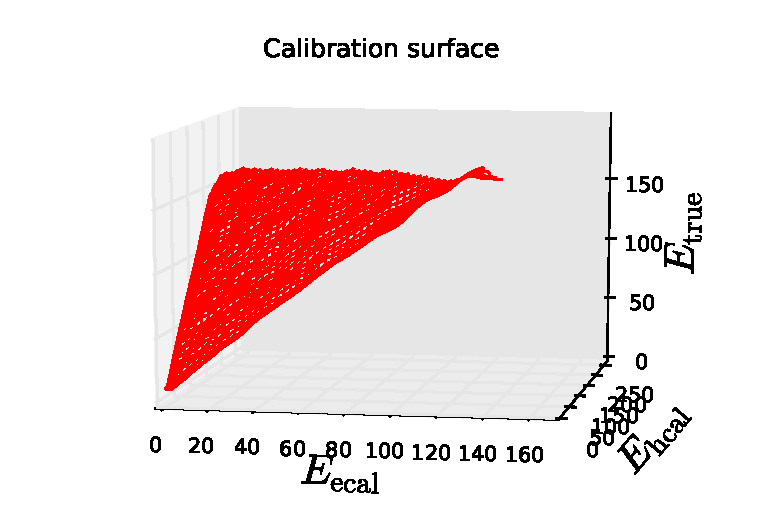
\includegraphics[width=\textwidth]{images/pictures/testKNN/KNN_plot3D_surf.eps}
	\captionof{figure}{Surface de calibration.}
	\label{surfKNN}
\end{minipage}

\begin{figure}[!h]
\begin{center}
\includegraphics[width=\textwidth]{images/pictures/testKNN/KNN_calibration.png}
\caption{Courbe de calibration pour $E_{\rm ecal} = 0$.}
\end{center}
\end{figure}

Nous constatons ici que la surface est beaucoup plus lisse qu'avec la méthode précédente, mais en regardant le cas particulier de $E_{\rm ecal} = 0$, nous constatons qu'une fois encore, à bas $E_{\rm hcal}$, la courbe de calibration ne passe pas par le coeur de la gerbe. Cela est dû à des points aberrants qui correspondent à des particules de haute énergie qui ne déposent pas ou peu leur énergie dans les calorimètres. Il faudra trouver un moyen de les écarter par la suite.

Effectuons alors la calibration d'un second jeu de données : 
\begin{figure}[!h]
\begin{center}
\includegraphics[width=\textwidth]{images/pictures/testKNN/KNN_ecalib_over_etrue.png}
\caption{$E_{\rm calib}/E_{\rm true}$ en fonction de $E_{\rm true}$.}
\label{ecaliboveretrueKNN}
\end{center}
\end{figure}

\begin{figure}[!h]
\begin{center}
\includegraphics[width=\textwidth]{images/pictures/testKNN/KNN_ecalib_over_etrue_functionof_ecal_hcal.png}
\caption{$E_{\rm calib}/E_{\rm true}$ en fonction de $E_{\rm ecal}$ et $E_{\rm hcal}$.}
\label{ecaliboveretrueKNN_ecal_hcal}
\end{center}
\end{figure}

Nous constatons que l'énergie de calibration est toujours sur-estimée, et particulièrement à bas $E_{\rm ecal}$ et $E_{\rm hcal}$ ( \textit{cf.} \ref{ecaliboveretrueKNN_ecal_hcal}).



\subsection{Nettoyage gaussien}
Cette méthode est assez similaire à la précédente. Elle se base sur la constatation que la distribution en énergie vraie des paquets de plus proches voisins est un distribution gaussienne. En utilisant la méthode des moindres carrés, nous allons donc  trouver les paramètres de la gaussienne en question et ne prendre en compte les plus proches voisins dont l'énergie vraie est $\mu -c\sigma \leq E_{\rm true}^i \leq \mu + c\sigma$ (nous prenons par défaut $c = 2$), avec $\mu, \sigma$ la moyenne et l'écart type de la distribution gaussienne.\\
Principe de l'algorithme :
\begin{itemize}
	\item on considère des points $(E_{\rm ecal}^{0,j}, E_{\rm hcal}^{0,j})$ où nous allons évaluer l'énergie calibrée.
	\item pour chaque $(E_{\rm ecal}^{0,j}, E_{\rm hcal}^{0,j})$ :
	\begin{itemize}
		\item on recherche ses $k$ plus proches voisins dans le plan $(E_{\rm ecal}, E_{\rm hcal}) \rightarrow (E_{\rm ecal}^i, E_{\rm hcal}^i), i \in [|1,...,k|]$
		\item on trouve la gaussienne correspondante $\mu -c\sigma \leq E_{\rm true}^i \leq \mu + c\sigma$
		\item on ne conserve que les voisins dont : $\mu -c\sigma \leq E_{\rm true}^i \leq \mu + c\sigma$
		\item on effectue une moyenne pondérée une moyenne pondérée de l'énergie vraie de ces plus proches voisins $\rightarrow E_{\rm calib}^0$ : l'énergie calibrée 
	\end{itemize}
	\item on effectue une interpolation pour donner une valeur d'énergie calibrée quelque soit $(E_{\rm ecal}^{0}, E_{\rm hcal}^{0})$
\end{itemize}


- on enlève les points éloignés du coeur de la distribution\\
- principe de l'algo\\
- comment fait-on un fit\\
-scipy \cite{scipyFit}\\
-{Efficacité du fit}:
\begin{figure}[!h]
\begin{center}
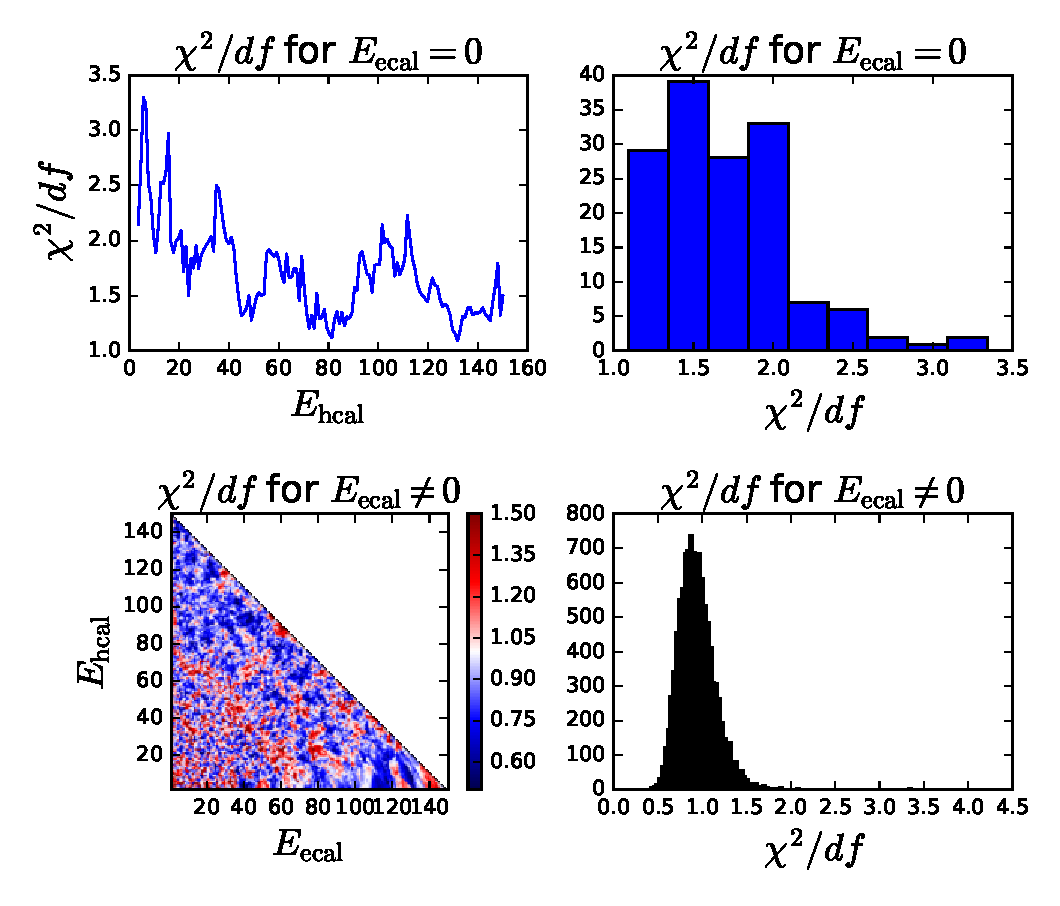
\includegraphics[width=0.7\textwidth]{images/pictures/testKNNGC/KNNGaussianCleaning_chi2_calib.eps}
\caption{Le $\chi^2$ réduit pour chaque fit effectué.}
\end{center}
\end{figure}
%	A différents moment, nous aurons besoin de calculer des moyennes. Or souvent, la moyenne classique ne serait pas représentative de ce que tous souhaitons montrer car certains points sont ont des valeurs $E_{\rm ecal},E_{\rm hcal}$ mal estimées car la simulation prend en compte les défauts des calorimètres. Il serait donc alors incorrecte de les prendre en compte pour juger l'efficacité d'une calibration car ils sont complètement incohérents.\\
%Pour résoudre ce problème, nous allons ajuster une gaussienne de la distribution des points à moyenner et choisir considérer que la moyenne à prendre en compte est la moyenne de la gaussienne. Ainsi, les points aberrants totalement écarté du centre de la distribution ne perturberont pas le calcul de la moyenne alors que dans le cas d'une moyenne classique, ils peuvent fortement attirer la moyenne vers eux.\\
%Ces points aberrants peuvent également venir d'une particule qui se serait décomposée avant le calorimètre. Ainsi on trouve près de l'origine, des points à fort $E_{\rm true}$ et pour de faibles valeurs de  $E_{\rm ecal}$ et $E_{\rm hcal}$, et ces points ne sont pas du tout représentatif de l'efficacité d'une calibration. 
%
%\begin{minipage}{0.5\linewidth}
%	\begin{center}
%	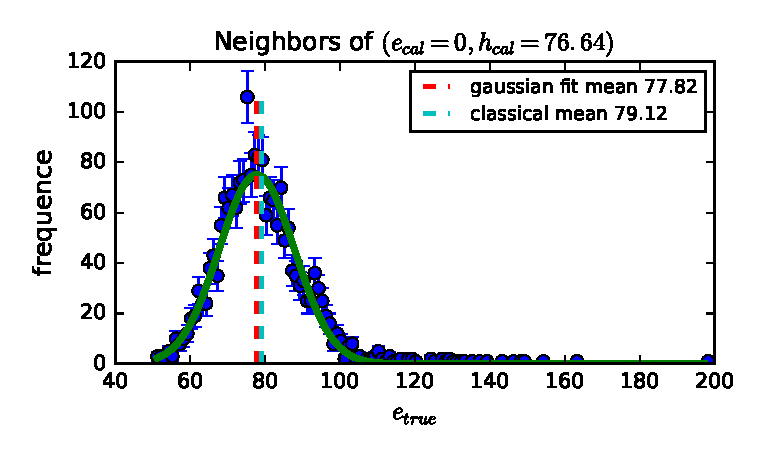
\includegraphics[height=5cm]{images/pictures/testKNNGF/KNNGaussianFit_example_hist.eps}
%	\end{center}
%\end{minipage}
%\hfill
%\begin{minipage}{0.45\linewidth}
%	Ici, on peut voir sur cet exemple que si nous prenons la moyenne classique de $E_{\rm true}$,  on obtient $79.12$, or la moyenne de la gaussienne fitée est de $77.82$, au vu de ce que nous avons dit précédemment, nous considèrerons que la seconde est plus judicieuse.
%\end{minipage}
%
%\subsection{Comment est fait un fit ?}
expliquer : \\
- barre d'erreur\\
- minimisation du chi2\\
- un bon chi2 réduit ?\\
- quand nous ferons un fit gaussien ce sera toujours le même principe\\
- interpolation \cite{scipyInterp}\\

\noindent
\begin{minipage}{0.6\linewidth}
Construisons alors la calibration  \cite{GitHubKNNGC} à l'aide des paramètres suivants : 
\[
\begin{cases}
\rm{lim} & = 150\\
n_{\rm neighbors, E_{\rm ecal} = 0} & = 2000\\
n_{\rm neighbors, E_{\rm ecal} \neq 0} & = 250\\
\rm{lim} & =150\\
\sigma  & = 5\\
\rm{weights} & = \rm{'gaussian'}\\
\rm{algorithm} & = \rm{'auto'}\\
\rm{energystep} & = 1\\
\rm{kind} & = \rm{'cubic'}\\
\rm{cut} & = 2\\
\end{cases}
\]
\end{minipage}
\begin{minipage}{0.4\linewidth}
	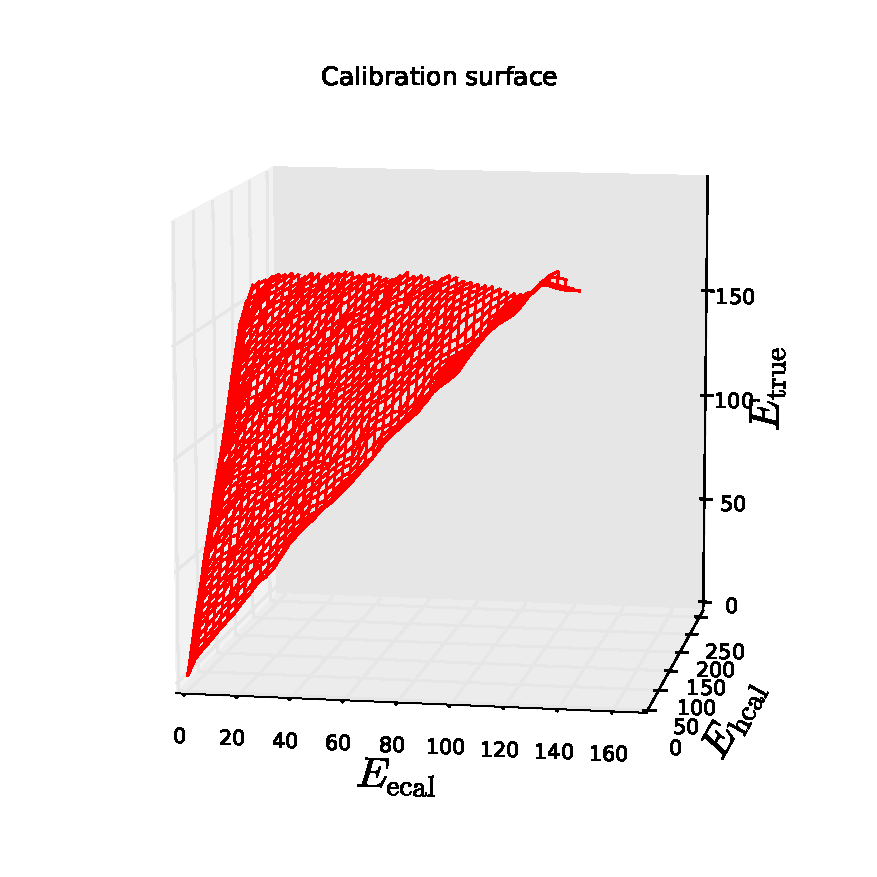
\includegraphics[width=\textwidth]{images/pictures/testKNNGC/KNNGaussianCleaning_plot3D_surf.eps}
	\captionof{figure}{Surface de calibration.}
	\label{surfKNNGC}
\end{minipage}

\begin{figure}[!h]
\begin{center}
\includegraphics[width=\textwidth]{images/pictures/testKNNGC/KNNGaussianCleaning_calibration.png}
\caption{Courbe de calibration pour $E_{\rm ecal} = 0$.}
\end{center}
\end{figure}

Effectuons alors la calibration d'un second jeu de données : 
\begin{figure}[!h]
\begin{center}
\includegraphics[width=\textwidth]{images/pictures/testKNNGC/KNNGaussianCleaning_ecalib_over_etrue.png}
\caption{$E_{\rm calib}/E_{\rm true}$ en fonction de $E_{\rm true}$.}
\label{ecaliboveretrueKNNGC}
\end{center}
\end{figure}

\begin{figure}[!h]
\begin{center}
\includegraphics[width=\textwidth]{images/pictures/testKNNGC/KNNGaussianCleaning_ecalib_over_etrue_functionof_ecal_hcal.png}
\caption{$E_{\rm calib}/E_{\rm true}$ en fonction de $E_{\rm ecal}$ et $E_{\rm hcal}$.}
\label{ecaliboveretrueKNNGC_ecal_hcal}
\end{center}
\end{figure}


\subsection{Fit gaussien}
Ici, il s'agit du même principe que précédemment mais nous allons considérer que la valeur de $E_{\rm calib}$ est la moyenne de la gaussienne. 
Principe de l'algorithme :
\begin{itemize}
	\item on considère des points $(E_{\rm ecal}^{0,j}, E_{\rm hcal}^{0,j})$ où nous allons évaluer l'énergie calibrée.
	\item pour chaque $(E_{\rm ecal}^{0,j}, E_{\rm hcal}^{0,j})$ :
	\begin{itemize}
		\item on recherche ses $k$ plus proches voisins dans le plan $(E_{\rm ecal}, E_{\rm hcal}) \rightarrow (E_{\rm ecal}^i, E_{\rm hcal}^i), i \in [|1,...,k|]$
		\item on trouve la gaussienne correspondante \rightarrow \sigma, \mu$
		\item $\rightarrow E_{\rm calib}^0 = \mu$
	\end{itemize}
	\item on effectue une interpolation pour donner une valeur d'énergie calibrée quelque soit $(E_{\rm ecal}^{0}, E_{\rm hcal}^{0})$
\end{itemize}

\noindent
\begin{minipage}{0.6\linewidth}
Construisons alors la calibration  \cite{GitHubKNNGF} à l'aide des paramètres suivants : 
\[
\begin{cases}
\rm{lim} & = 150\\
n_{\rm neighbors, E_{\rm ecal} = 0} & = 2000\\
n_{\rm neighbors, E_{\rm ecal} \neq 0} & = 250\\
\rm{lim} & =150\\
\rm{algorithm} & = \rm{'auto'}\\
\rm{energystep}_{E_{\rm ecal} = 0} & = 1\\
\rm{energystep}_{E_{\rm ecal} \neq 0} & = 5\\
\rm{kind} & = \rm{'cubic'}\\
\end{cases}
\]
\end{minipage}
\begin{minipage}{0.4\linewidth}
	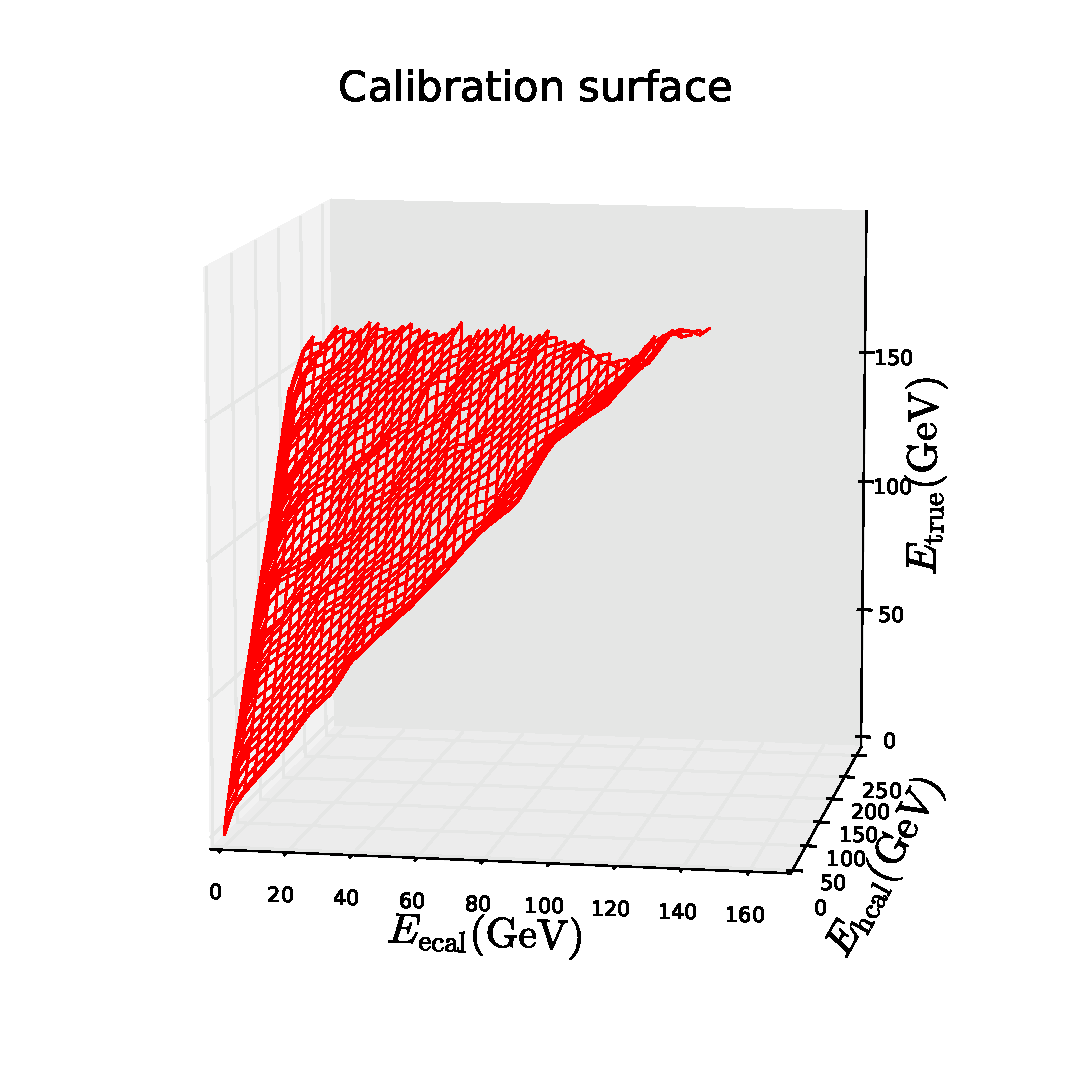
\includegraphics[width=\textwidth]{images/pictures/testKNNGF/KNNGaussianFit_plot3D_surf.eps}
	\captionof{figure}{Surface de calibration.}
	\label{surfKNNGF}
\end{minipage}
\begin{figure}[!h]
\begin{center}
\includegraphics[width=\textwidth]{images/pictures/testKNNGF/KNNGaussianFit_calibration.png}
\caption{Courbe de calibration pour $E_{\rm ecal} = 0$.}
\end{center}
\end{figure}

Effectuons alors la calibration d'un second jeu de données : 
\begin{figure}[!h]
\begin{center}
\includegraphics[width=\textwidth]{images/pictures/testKNNGF/KNNGaussianFit_ecalib_over_etrue.png}
\caption{$E_{\rm calib}/E_{\rm true}$ en fonction de $E_{\rm true}$.}
\label{ecaliboveretrueKNNGF}
\end{center}
\end{figure}

\begin{figure}[!h]
\begin{center}
\includegraphics[width=\textwidth]{images/pictures/testKNNGF/KNNGaussianFit_ecalib_over_etrue_functionof_ecal_hcal.png}
\caption{$E_{\rm calib}/E_{\rm true}$ en fonction de $E_{\rm ecal}$ et $E_{\rm hcal}$.}
\label{ecaliboveretrueKNNGF_ecal_hcal}
\end{center}
\end{figure}


\section{Comparaison des méthodes}
\label{comparaison}
\subsection{Méthodes des plus proches voisins}
%\begin{figure}[!h]
%\begin{center}
%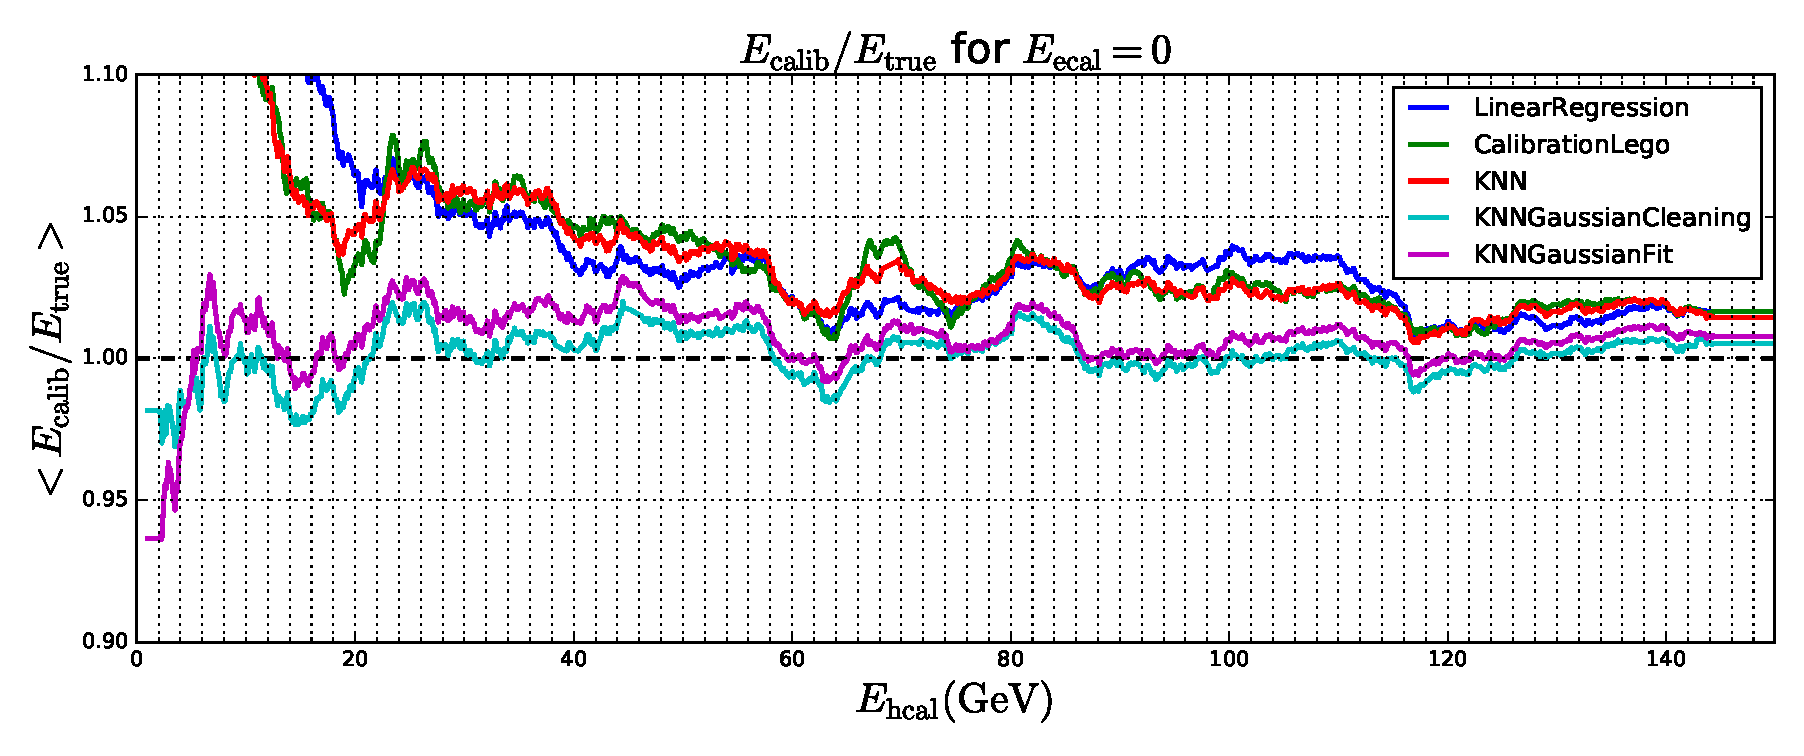
\includegraphics[width=\textwidth]{images/pictures/comparisons/comparison1.eps}
%\caption{$E_{\rm calib}/E_{\rm true}$ en fonction de $E_{\rm true}$.}
%\end{center}
%\end{figure}
%
%
%\section{Meilleure méthode}
%\begin{figure}[!h]
%\begin{center}
%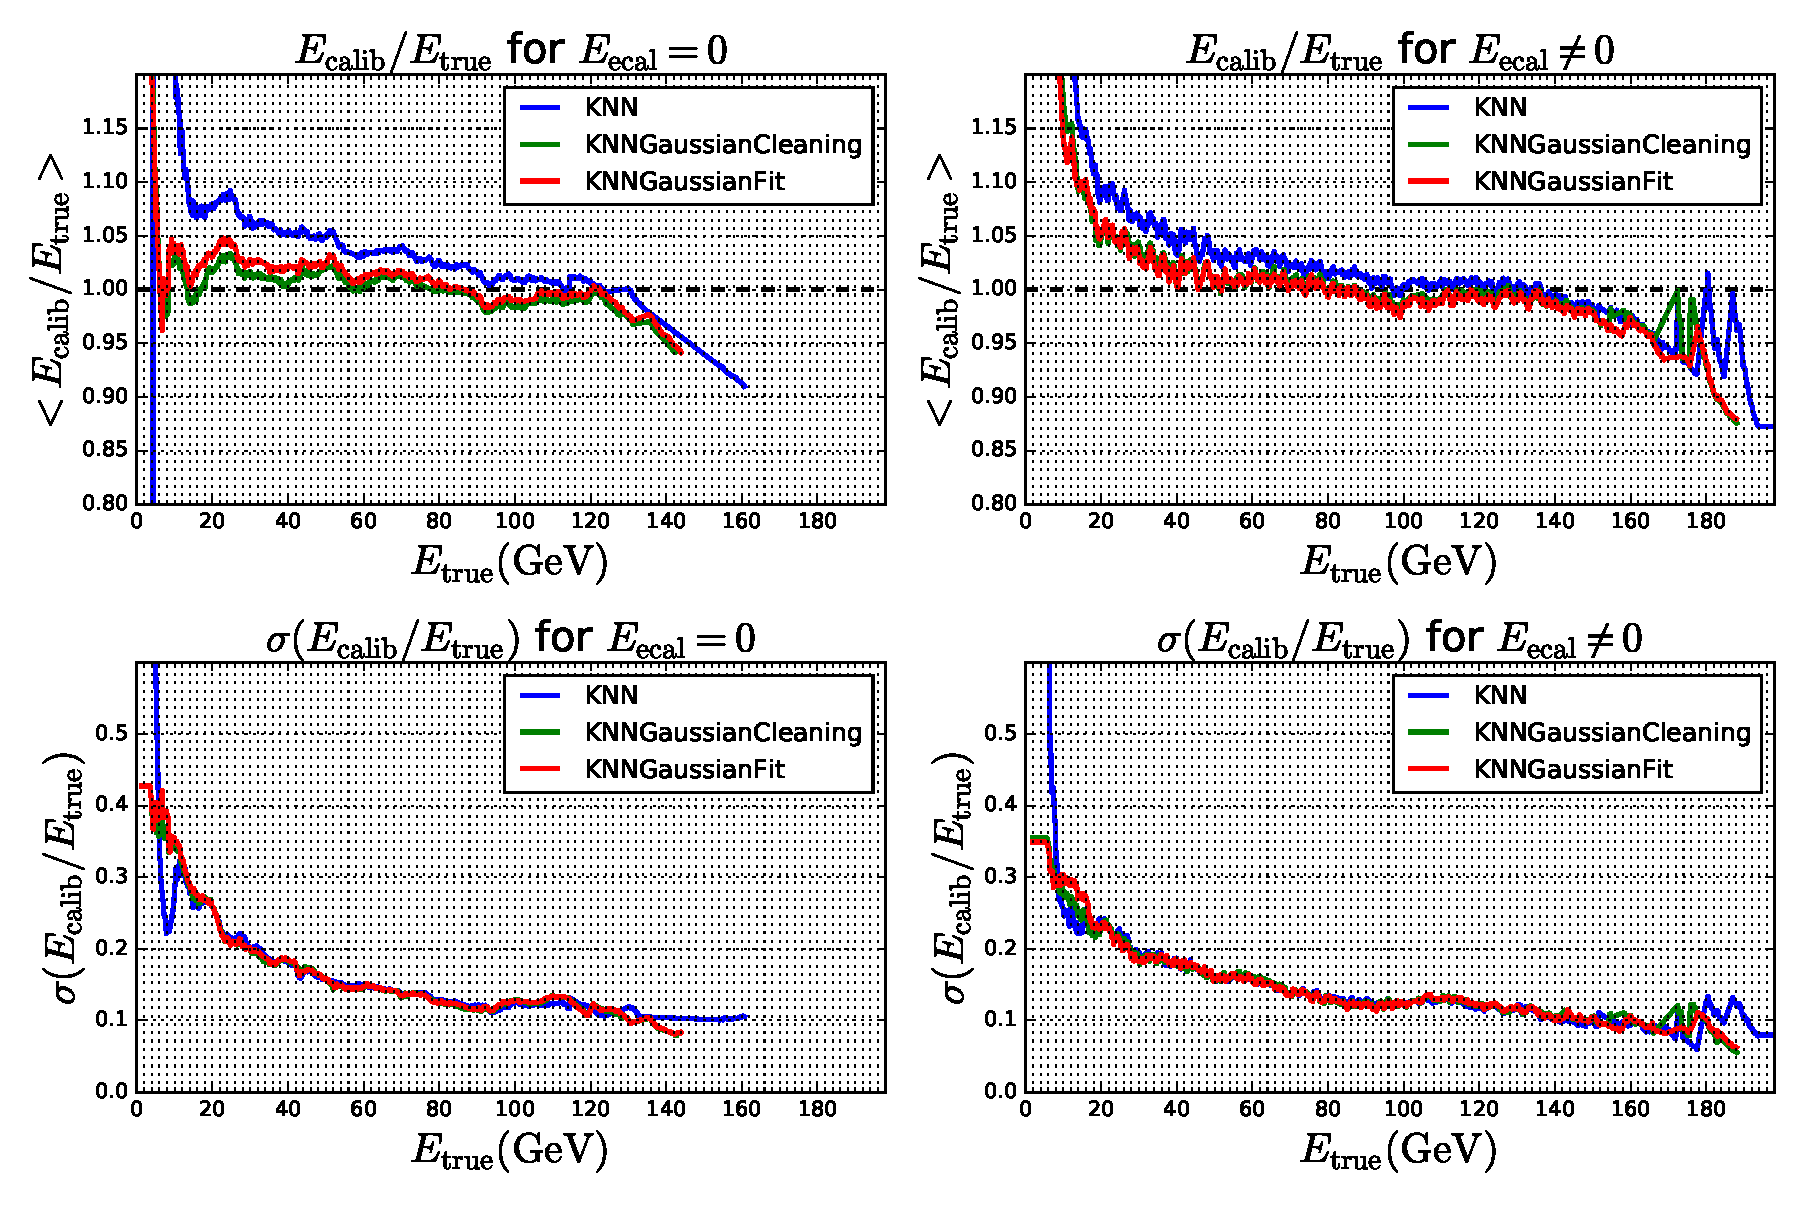
\includegraphics[width=\textwidth]{images/pictures/comparisons/comparison2.eps}
%\caption{$E_{\rm calib}/E_{\rm true}$ en fonction de $E_{\rm true}$.}
%\end{center}
%\end{figure}
%
%
%
%

\section{Annexes}
\subsection{Fonctions utiles du programme}

\newpage
\bibliographystyle{unsrt}
\bibliography{biblio} % mon fichier de base de données s'appelle biblio.bib

\end{document}

